% ==> roboust externalize test
\InputIfFileExists{ztikz-cfg.tex}{}{}
\documentclass{article}
% \usepackage{robust-externalize}
% \cacheEnvironment{tikzpicture}{tikzpicture}
\usepackage{xcolor}
\usepackage{tikz}
\usepackage{xsimverb}
\usepackage{ztool}
\usepackage{xparse}
% \usepackage{ztikz}
% \usetikzlibrary{external}
% \tikzset{external/up to date check={diff}}
% \tikzexternalize[prefix=tikz-cache/]

\makeatletter
\ExplSyntaxOn
% NOT compatible with 'external' library
\tl_new:N \l_ztikz_cache_forward_value_tl
\str_new:N \l_ztikz_cache_forward_name_str
\keys_define:nn {ztikz/cache}
  {
    delimiter  .tl_set:N    = \l_ztikz_cache_arg_delimiter_tl,
    delimiter  .initial:n   = { [] },
    forward    .clist_set:N = \l_ztikz_cache_forward_clist,
    forward    .initial:n   = { \empty },
  }
\cs_new:Npn \__ztikz_cache_deps:n #1 
  {
    \c_percent_str\exp_not:n {#1}:=~#1^^J
  }
\NewDocumentCommand{\ztikzCacheEnv}{om}
  {% #1:new arg-spec; #2:ori-env name; 
  % !! Only single optional arg is permitted
    \DeclareEnvironmentCopy{ztikz@cached@#2}{#2}
    \IfValueT{#1}{ \keys_set:nn {ztikz/cache}{#1} }
    \exp_args:Nne \DeclareDocumentEnvironment{#2}{D\l_ztikz_cache_arg_delimiter_tl{}}
      {% No arg: line content locates at '\begin{<ENV>}' will be gobbled
        % \typeout{--->##1} % --->Mand
        % \typeout{--->##2} % --->HHJKHJKHJ
        % \GetDocumentEnvironmentArgSpec {#2}
        % \typeout{--->\ArgumentSpecification} % --->O{HELLO}mm
        \tl_if_empty:VTF \l_ztikz_cache_arg_delimiter_tl
          { \xsim_file_write_start:nn {\c_true_bool}{ZZZ.tex}\typeout{-->empty~arg} }
          { \xsim_file_write_start:nn {\c_false_bool}{ZZZ.tex} }
      }{
        \xsim_file_write_stop:
        \ztool_insert_to_file:nnn {ZZZ.tex}{1}
          {
            \clist_map_function:NN 
              \l_ztikz_cache_forward_clist 
              \__ztikz_cache_deps:n 
            \exp_not:N\begin{ztikz@cached@#2}
              \tl_item:Nn \l_ztikz_cache_arg_delimiter_tl {1}
              ##1
              \tl_item:Nn \l_ztikz_cache_arg_delimiter_tl {-1}
          }
        \ztool_append_to_file:nn {ZZZ.tex}
          { \exp_not:N \end{ztikz@cached@#2} }
        % \exp_args:No \begin{ztikz@cached@#2}\l_ztikz_cache_arg_delimiter_tl
        % \end{ztikz@cached@#2}
      }
  }
% \ztool_insert_to_file:nnn {temp-w.txt}{3}{NEW-LINE}

% \NewDocumentEnvironment{example}{o}
%   {
%     \IfNoValueTF{#1}
%       {\XSIMfilewritestart*{\jobname-s.txt}}
%       {\XSIMfilewritestart{\jobname-s.txt}}%
%   }{\XSIMfilewritestop}
% \AddToHook{env/ctikzpicture/before}{\begin{example}\begin{ctikzpicture}{Mand}{HHJKHJKHJ}}
% \AddToHook{env/ctikzpicture/after}{\end{example}}
\ExplSyntaxOff
\ztikzCacheEnv[delimiter=[], forward={\AAA,\empty}]{tikzpicture}


\begin{document}
\def\AAA{AAA-aba}

BBB \AAA{} bbb.

% I am a cached picture: \begin{tikzpicture}<forward=\AAA>
% \node[draw,rounded corners,fill=teal!50](A){BBB \AAA{} bbb.};
% \end{tikzpicture}.

% \begin{tikzpicture}
%   \node[draw,rounded corners,fill=teal!50](A){BBB \AAA{} bbb.};
% \end{tikzpicture}

% \pdfmdfivesum file {XXX.tex}
% AAA-aaa. 8CFC240350E96BB198E39BF0C450A522
% AAA-aba. 1425867299391550907B35C5C8C66BD8
% comment check 1: 3CA4F9C40B4A161FDB92DA4E0FD7B89C
% comment check 2: D0B16CF7620A6B4EF806FB3C8228C55B

% \begin{tikzpicture}
%   \node[draw,rounded corners,fill=teal!50](A){BBB \AAA{} bbb.};
% \end{tikzpicture}

\def\BBB{BBB-bbb}
% \begin{example}
% \begin{ctikzpicture}{Mand}{HHJKHJKHJ}
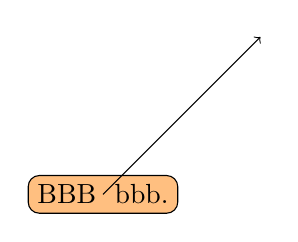
\begin{tikzpicture}[scale=2]
  \node[draw,rounded corners,fill=orange!50](A){BBB \AAA{} bbb.};
  \draw[->] (0, 0) -- (1, 1)node {\BBB};
\end{tikzpicture}
% \end{example}

% \ShowDocumentEnvironmentArgSpec {tikzpicture}
% \typeout{--->\ArgumentSpecification} % --->mm

%\AAA := AAA-aba
%\empty :=
\begin {ztikz@cached@tikzpicture}[scale=2]

  \node[draw,rounded corners,fill=orange!50](A){BBB \AAA{} bbb.};
  \draw[->] (0, 0) -- (1, 1)node {\BBB};
\end {ztikz@cached@tikzpicture}



% --> extract preable on the fly
% \ExplSyntaxOn
% \ztool_gread_file_as_seq:nnN {\c_true_bool}{debug.tex}{\l_tmpa_seq}
% % \seq_show:N \l_tmpa_seq
% \prg_generate_conditional_variant:Nnn \str_if_eq:nn { ne } { TF }
% \prg_generate_conditional_variant:Nnn \str_if_empty:n { e } { F }
% \str_set:Nn \l_tmpa_str {\begin{document}}
% \iow_open:Nn \g_ztool_file_append_iow {extract-preamble.tex}
% \seq_map_inline:Nn \l_tmpa_seq 
%   {
%     \str_if_eq:neTF {#1}{\l_tmpa_str}
%       { 
%         \seq_map_break: 
%         \iow_close:N \g_ztool_file_append_iow
%       }
%       % { \seq_put_right:Nn \l_tmpb_seq {#1} }
%       { 
%         \str_if_empty:eF {\tl_trim_spaces:n {#1}}{
%         \iow_now:Ne \g_ztool_file_append_iow 
%           { \exp_not:n {#1}}
%         }
%       }
%   }
% % \seq_show:N \l_tmpb_seq
% \ExplSyntaxOff
\end{document}




% ===> ApTeX Test
% NOTE:
% 1.'dvipdfm' and 'dvipdfmx' can get graphics dimension
% 2.'dvpdfm' do NOT support fadings
% 3.NOT compatiable with tikz 'external' library
% REF: https://tex.stackexchange.com/a/17737/294585
\InputIfFileExists{ztikz-cfg.tex}{}{}
\documentclass{article}
\def\pgfsysdriver{pgfsys-dvipdfmx.def}
\usepackage[dvipdfmx]{graphicx}
\usepackage{ztikz}
\ztikzloadlibrary{gnuplot, zdraw}


\begin{document}
\section{Normal picture}
\begin{figure}[!htb]
  \centering
  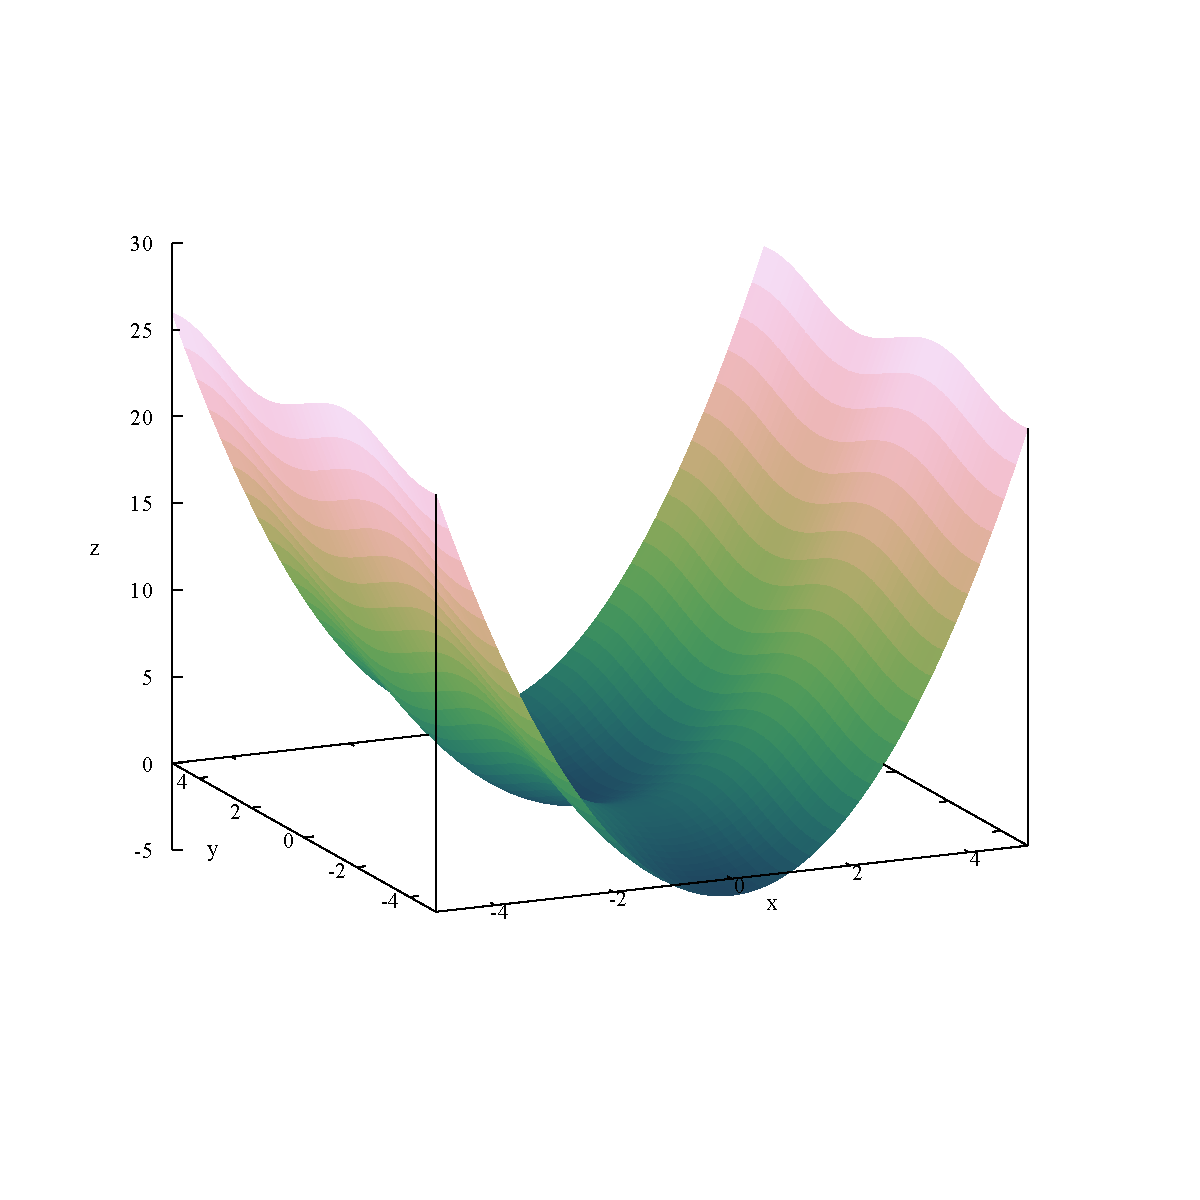
\includegraphics[width=.75\linewidth]{./pics/plot_3d_1.pdf}
  \caption{AAA}
  \label{fig:AAA}
\end{figure}

\section{tikz}
\subsection{builtin}
\begin{tikzpicture}
  \draw[very thin,color=gray] (-0.1,-1.1) grid (3.9,3.9);
  \draw[->] (-0.2,0) -- (4.2,0) node[right] {$x$};
  \draw[->] (0,-1.2) -- (0,4.2) node[above] {$f(x)$};
  \draw[color=red] plot (\x,\x) node[right] {$f(x) =x$};
  % \x r means to convert '\x' from degrees to _r_adians:
  \draw[color=blue] plot (\x,{sin(\x r)}) node[right] {$f(x) = \sin x$};
  \draw[color=orange] plot (\x,{0.05*exp(\x)}) node[right] {$f(x) = \frac{1}{20} \mathrm e^x$};
\end{tikzpicture}


\subsection{ztikz}
\begin{tikzpicture}
\ShowGrid{(-5, -5);(5, 5)}
\Plot[
  domain=0:2*pi, 
  style={color=teal}, 
  marker={type=square*, color=red, rotate=45}
]{2*sin(x)}
\ContourPlot[
  domain={-1.5:1.5;}, 
  style={color=red}, 
]{x**2/4+y**2-1}
\PlotPrecise{param}{100}
\ParamPlot[domain=-pi:pi, style={teal, very thick}]{4*sin(t), 2*cos(t)}
\PolarPlot{2*(1-sin(t))}
\end{tikzpicture}

\subsection{gnuplot}
\Plotz[palette={cubehelix start 0 cycles -1. saturation 1}]{x**2-sin(y)}


\section{l3draw Test}
NOT SUPPORT YET

% \begin{center}
%   \zrule[width=10, startColor=red, step=0.5]
% \end{center}

% \ExplSyntaxOn
% \cs_set_eq:NN \moveto:n \draw_path_moveto:n
% \cs_set_eq:NN \gdraw:n  \draw_path_use_clear:n
% \draw_begin:
%   \int_step_inline:nnnn {0}{45}{360}{
%     \draw_path_circle:nn {
%       \draw_point_polar:nn {2em}{#1}
%     }{2pt}
%   }
%   \gdraw:n {fill}
% \draw_end:
% \ExplSyntaxOff
\end{document}


% ==> hash char catcode
\InputIfFileExists{ztikz-cfg.tex}{}{}
\documentclass{article}
\usepackage{ztool}



\begin{document}
\ExplSyntaxOn
\group_begin:
\char_set_catcode_other:N \#
% \char_set_catcode_other:n { 35 }

% \tl_set_eq:NN \l_tmpa_tl \c_hash_str
\gdef\hashchar{#}
\group_end:

% \ztool_append_to_file:nn {temp-w.txt}
%   {\exp_not:n {#}}

\tl_set:Nn \l_tmpa_tl {\exp_not:n {#1}}
\tl_show:N \l_tmpa_tl
\ExplSyntaxOff


Hello world: \hashchar{} HAHA
\end{document}





% ===> test gif insert
\documentclass{article}
\usepackage{graphicx}
\usepackage{animate}


\begin{document}
\begin{center}
  \animategraphics[
    loop,controls,
    width=.75\linewidth
  ]{10}{./pics/gif/test-gif-converted-to-}{0}{}
\end{center}
\end{document}



\documentclass{article}
\usepackage{graphicx}
\usepackage{epstopdf}
% \epstopdfDeclareGraphicsRule
%   {.gif}{png}{.png}{convert gif:test.gif png:TEST}
\DeclareGraphicsRule{.gif}{png}{.png}{`convert #1 `basename #1 .gif`-gif-converted-to.png}
\AppendGraphicsExtensions{.gif}


\begin{document}
Hello world.

\begin{figure}[!htb]
  \centering
  
\includegraphics[width=.75\linewidth]{test.gif}
  \caption{}
  \label{fig:}
\end{figure}

\end{document}





% ==> test sed replacement
\InputIfFileExists{ztikz-cfg.tex}{}{}
\documentclass{article}
\usepackage{ztikz}
\ztikzloadlibrary{cache, gnuplot}


\begin{document}
\begin{tikzpicture}
\ShowGrid{(-5, -5);(5, 5)}
\Plot[
  domain=0:2*pi, 
  style={color=teal}, 
  marker={type=square*, color=red, rotate=45}
]{2*sin(x)}

\ContourPlot[
  domain={-1.5:1.5;}, 
  style={color=red}, 
]{x**2/4+y**2-1}
\PlotPrecise{param}{6}
\ParamPlot[domain=-pi:pi, style={teal, very thick}]{4*sin(t), 2*cos(t)}
\PolarPlot{2*(1-sin(t))}
\end{tikzpicture}

\Plotz[palette={cubehelix start 0 cycles -1. saturation 1}]{x**2-sin(y)}
\end{document}


% ==> test
\InputIfFileExists{ztikz-cfg.tex}{}{}
\documentclass{article}
\usepackage{graphicx}
\usepackage{amsmath}
\usepackage{ztikz}
\ztikzloadlibrary{cache, python, wolfram}
% \ztikzloadlibrary{wolfram}


\begin{document}
% \ExplSyntaxOn
% \ztool_append_to_file:nn {temp.txt}{XXX-1}

% \ztool_append_to_file:nn {temp.txt}{XXX-2}
% \ExplSyntaxOff

% \begin{pyfig}[width=.45\linewidth]{pycode.py}
% import matplotlib
% matplotlib.use('Agg')
% from matplotlib import pyplot as plt
% plt.rcParams['font.sans-serif'] = ['FangSong']
% plt.rcParams['axes.unicode_minus'] = False
% import numpy as np
% x = np.linspace(0, 2*np.pi, num = 80)
% y = np.sin(x)*np.cos(x)+.2
% plt.plot(x, y, 'ro')
% \end{pyfig}

% \[
%   2^{64} = \py{2**64}
% \]
\begin{wolframGraphics}
FIGURE=Plot[Sin[x], {x, -Pi, Pi}]
\end{wolframGraphics}

\begin{figure}[!htb]
  \centering
  \includegraphics[width=.75\linewidth]{\wolframOuputFile}
  \caption{Wolfram-Ouput-FIGURE}
  \label{fig:Wolfram-Ouput-FIGURE}
\end{figure}

\begin{wolframGraphics}[width=.5\linewidth]
  FIGURE=Plot[Sin[x], {x, -Pi, Pi}]
\end{wolframGraphics}

\wolfram{LaplaceTransform[t^4 Sin[3*t], t, s]}
\[
  \wolframResult
\]

\wolfram{2+2}
\[
  \wolframResult
\]

\wolframSolve[var={x, y}]{a x + y == 8 && b x - y == 1}
\begin{align}
  &  \wolframResult \\
  &  \wolframResult[||] \\
  &  \wolframResult* \\
  &  \wolframResult*[3-1]\\
  &  \wolframResult*[-1] \\
  &  \wolframResult*[a]
\end{align}

\wolframSolve[var={x, y}, domain=Integers]{x^2 + 2 y^3 == 3681 && x > 0 && y > 0}
\begin{align}
  \wolframResult
\end{align}


\wolframSolve[var={x, y}, domain=Integers]{x+y == 5 && x > 0 && y > 0}
\begin{align}
  &\wolframResult[\\&]
\end{align}


\wolframDSolve{y'[x] + y[x] == a*Sin[x], y[0] == 1}
\begin{align}
  &\wolframResult
\end{align}

\wolframDSolve[depend={y[x], z[x]}]{y'[x] == Exp[z[x]] + 1, z'[x] == y[x] - x}
\begin{align}
  &\wolframResult[\\&]
\end{align}
\end{document}


% ==> append to file
\InputIfFileExists{ztikz-cfg.tex}{}{}
\documentclass{article}
\usepackage{../../ztool/code/ztool}


\begin{document}
\ExplSyntaxOn
\ior_new:N \g_file_append_ior
\iow_new:N \g_file_append_iow
\str_new:N \l_file_content_str
\str_clear:N \l_file_ori_content_str
\cs_new:Npn \c_hash_symbol   {\iow_char:N \# }
\cs_new:Npn \c_space_symbol  {\iow_char:N \  }
\cs_new_protected:Npn \__append_to_file:nn #1#2 
  {% #1: file name; #2: content
    \ior_open:Nn \g_file_append_ior {#1}
    \ior_str_map_inline:Nn \g_file_append_ior
      {
        \str_put_right:Nx \l_file_ori_content_str {^^J\tl_to_str:n {##1}}
      }
    \iow_open:Nn \g_file_append_iow {#1}
    \str_remove_once:Nn \l_file_ori_content_str {^^J}
    \iow_now:Ne \g_file_append_iow {\l_file_ori_content_str} 
    \tl_set:Nn \l_tmpa_tl {#2}
    \tl_set_rescan:Nnn \l_tmpa_tl 
      {
        % \cctab_select:N \c_str_cctab
        \char_set_catcode_letter:n {35}
        \char_set_catcode_letter:n {36}
        \char_set_catcode_letter:n {64}
        % \char_set_catcode_letter:n {92}
        \char_set_catcode_letter:n {94}
        \char_set_catcode_letter:n {95}
        % \char_set_catcode_other:N \exp_not:N \~
      }{#2}
    \iow_now:Ne \g_file_append_iow {\l_tmpa_tl}
    \iow_close:N \g_file_append_iow
  }

% \newcommand{\test}{\c_hash_str/$<~ \c_backslash_str@2_#^1>\c_backslash_str *$\c_hash_str|}
\__append_to_file:nn {temp.txt}{ABCD~ EFG}
  
% \ztool_append_to_file:nn {temp.txt}
%   {\c_hash_str/$<~ \c_backslash_str@2_#^1>\c_backslash_str *$\c_hash_str|}
\ExplSyntaxOff

HELLO
\end{document}




\InputIfFileExists{ztikz-cfg.tex}{}{}
\documentclass{article}
\usepackage{ztikz}
\usepackage{xsimverb}
\ztikzloadlibrary{gnuplot}
\ExplSyntaxOn
\newcommand{\xsimStart}[1]{
  \xsim_file_write_start:nn {\c_true_bool}{#1}
}
\newcommand{\xsimEnd}{\xsim_file_write_stop:}

\newenvironment{export}[1]{
  \xsim_file_write_start:nn {\c_false_bool}{#1}
  \gdef\filename{#1}
}{
  \xsim_file_write_stop:
  \expandafter\input\expandafter{\filename}
}
\ExplSyntaxOff
% \AddToHook{env/tikzpicture/before}{\begin{export}{XXX.tex}}
% \AddToHook{env/tikzpicture/after}{\end{export}}


\begin{document}
\section{gnuPlot}
\PlotPrecise{plot}{50}


\def\AAA{aaa}
% \begin{export}{export-2.tex}
\begin{tikzpicture}
  \Plot[
    domain=0:2*pi, 
    style={color=teal}, 
    % marker={type=square*, color=red, rotate=45}
  ]{2*sin(x)}
  \StemPlot[x][red][type=*, color=orange]{\gnudata{1}}
  \node at (0, 0) {\AAA};
\end{tikzpicture}
% \end{export}

% \show\tikzpicture
\end{document}